\cleardoublepage
\chapter{Learning MPC controllers with pQP neural networks}
\markboth{Learning MPC controllers with pQP neural networks}{Learning MPC controllers with pQP neural networks}

\section{Introduction}

Consider the standard MPC formulation for linear dynamical systems
\begin{subequations}
	\label{eq:linearmpc}
	\begin{align}
		%\mathds{P}1: \min_{X,U} \quad & q(x_H) + \sum_{k=1}^{H-1} l(x_k,u_k) \\
		\mathds{P}1: \min_{X,U} \quad & \sum_{k=0}^{N-1} \big( x_k^\top Q x_k + u_k^\top R u_k \big) + x_N^\top P x_N\\
		\text{subj. to} \quad 
		& x_{k+1} = A x_{k} + B u_{k}, \, \forall k = 0,\dots,N-1  \\
		& x_{k} \in \mathbb{X}, \, \forall k = 0,\dots,N-1 \\
		& u_{k} \in \mathbb{U}, \, \forall k = 0,\dots,N-1 \\
		& x_{H} \in \mathbb{X}_N \\
		& x_0 = x(0)
	\end{align}
\end{subequations}
where $x_k \in \mathbb{R}^{n_x}$, $u_k \in \mathbb{R}^{n_u}$, for all $k$; $X:=\{x_1,\dots,x_{N}\}$ and $U:=\{u_0,\dots,u_{N-1}\}$ are the collections of decision variables; $Q \succeq 0$, $R \succeq 0$ and $P \succ 0$ are cost matrices of adequate size; and the sets $\mathbb{X}$, $\mathbb{X}_N$ and $\mathbb{U}$ are polyhedra. Also, denote by 
\begin{equation}
	\pi: \mathcal{X} \rightarrow \mathbb{U}, \quad x(0) \mapsto \pi(x(0)) = u_0^\star
\end{equation} 
the mapping defined point-wise from the parameter $x(0)$ of $\mathds{P}1$ to the first control component of its optimizer\footnote{Since the objective is strictly convex and the constraints define a convex feasible set, if an optimizer exists for a given parameter $x(0)$, then this optimizer is unique.}. The domain $\mathcal{X} \subset \mathbb{R}^{n_x}$ is the collection of all $x(0)$ for which $\mathds{P}1$ is finite, i.e., the problem is feasible. It is well-known that, under reasonable standard on the terminal ingredients $P$ and $\mathbb{X}_N$, the map $\pi$ is a piece-wise affine continuous function over a polyhedral partition of the polyhedron $\mathcal{X}$ \citep{bemporad2002explicit,borrelli2017predictive}. 

Automatic control involves real-time decision making and, in a number of different scenarios, it becomes infeasible or simply undesirable to solve an optimization problem such as \eqref{eq:linearmpc} on-line. Picture, for instance, a small embedded system that does not have enough computational resources to arrive at a solution within the time allocated to it. One method to circumvent solving $\mathds{P}1$ is to seek $\pi$, which can explicitly written in closed form with multi-parametric programming tools \citep{bemporad2002explicit}. This approach is known as explicit MPC and has become an establish control tool \citep{mariethoz2008explicit,naus2010design} for which free software exists \citep{herceg2013multi}. Unfortunately, $\pi$ can also be challenging both to compute and to store as the number of regions of its domain grows exponentially in the worst case with the number of inequality constraints in $\mathds{P}1$ \citep{alessio2009survey}, thus limiting its applicability. Simplifications strategies for explicit MPC exist, each coming with a different set (sometimes empty) of guarantees. In \cite{geyer2008optimal} and \cite{wen2009analytical}, for example, the authors build equivalent but more convenient representations of the control policy; in \cite{jones2008double} an incremental method is proposed to fit $\pi$ without requiring its explicit description; and in \cite{christophersen2007controller} and \cite{maddalena2019robust} safe elimination procedures are presented to drop certain regions without disrupting certain closed-loop properties.

%We assume a set of $N$ samples can be acquired from the original control law\footnote{The dataset can also be directly obtained from the implicit controller; depending on the size of the problem at hand, computing the explicit solution might be intractable.}
%\begin{subequations}
%	\begin{align}
%		& D = \{\text{x}_i,\text{u}_i\}_{i=1}^{N} \\[3pt]
%		& \text{u}_i = \pi(\text{x}_i), \; i=1,\dots,N
%	\end{align}
%\end{subequations}
%The process of acquiring the training dataset does not have to follow a particular distribution, nor do the samples have to be independent.

With the recent popularization of deep learning and the plethora of easy-to-use toolboxes available to users, neural network (NN) approximations of the map linking the current state $x(0)$ to the MPC optimal control action $u_0^\star$ have also become trendy (see e.g. \cite{karg2020efficient,kumar2021industrial}). Although the idea itself is not new \citep{parisini1995receding}, the latest investigations tend to make use of more modern analysis and synthesis tools such as better activation functions and training algorithms. The works \cite{fazlyab2020safety} and \cite{schwan2022stability} address the problem of verifying a NN approximation a posteriori, employing respectively semi-definite and mixed-integer linear programming techniques. On a different spirit, \cite{paulson2020approximate} tackles designing NNs that approximate predictive controllers and are safe by design. Arguably the main motivation behind this entire line of research is the expressive power of NNs, especially when deep architectures are employed \cite{karg2020efficient}, and the fact that they lie in the same class of piece-wise affine (PWA) functions as MPC controllers\footnote{As long as a PWA activation function such as the rectified linear unit (ReLU) is used.}.

As opposed to the previously cited works where rather multi-purpose NN architectures were used, we will explore a structure that is tailored to the problem $\mathds{P}1$ and its solution $\pi$. Our proposal, which was published in \cite{maddalena2020neural} and \cite{maddalena2021embedded}, revolves around utilizing convex programs as layers within neural networks as proposed in \cite{amos2017optnet} and \cite{agrawal2019differentiable}. More specifically, the parameter to optimizer map of a convex program is employed as an internal layer, offering a particular inductive bias. A shallow architecture is proposed and shown to be able to represent the map $\pi$ of any predictive controller \eqref{eq:linearmpc} given a sufficiently large size. Finally, two examples are presented in the area of power electronics, allowing for a drastic speed-up in computation times with only a minor performance degradation.
	
\subsection{The proposed architecture}

An illustration of the parametric quadratic program (pQP) neural network is shown in Figure~\ref{fig:nnArchitecture}. It is composed of two linear layers (L1 and L3), a single non-linear layer with adjustable parameters (L2), and a fixed output layer (L4). The central part of this structure is the pQP layer L2, which is an implicit function described by the optimization model
%The key idea behind the proposed approximator is the use of a parametric quadratic program layer as part of the Neural Network, and optimizing over its parameters in order to fit the available dataset. This layer is implicitly described by the quadratic program
\begin{equation}
	\label{eq:pQP}
	y_2 = \text{arg}\,\min_{z \geq 0} \; ||Hz + y_1||^{2} + \epsilon ||z||^2
\end{equation}
that has $y_1$, the output of layer L1, as a parameter; the optimizer $y_2$ is then a function of $y_1$. Note how \eqref{eq:pQP} is always feasible and bounded from below, thus well posed for any $y_1$. The regularizing constant $\epsilon > 0$ is a fixed parameter that contributes with the numerical stability of the scheme. Additionally, if $\epsilon > 0$, then \eqref{eq:pQP} has always a unique minimizer and thus the map $y_1 \mapsto y_2$ is well defined.

Intuitively, one can think of the first layer L1 as a lifting, or projection, of the current state $x \in \mathbb{R}^{n_x}$ onto another space $\mathbb{R}^{n_z}$ whose dimension is a NN hyperparameter to be chosen by the user. L2 then is the key non-linear transformation that should capture most of the MPC policy complexity. Next, the affine map in L3 takes the $y_2$ value to the input space $\mathbb{R}^{n_u}$ and finally the control actions are guaranteed to satisfy the control constraints by projecting them onto $\mathbb{U}$, which is accomplished by L4 (see \eqref{def.pol_proj}). By adjusting $n_z$, the designer increases or reduces the representation power of the pQP NN although its size remains constant.
%which is \textit{always feasible} and \textit{bounded from below}. The size of this mathematical program, i.e. the dimension of $z$, can be tuned to attain approximations with different complexity. Moreover, as notation suggests, the parameter $y_1$ depends on a previous affine layer that maps the system states into the $z$ space, $y_1 := Fx + f$. Let $y_2 := z^{\star}$, then another affine layer maps the optimal solution to the input space $y_3 := Gy_2 + g$, and a projection onto the feasible input set produces the final control action $\hat{u} := \text{Proj}_{\, \mathbb{U}}(y_2)$. This last step is necessary to guarantee feasibility of the control moves (see e.g. \cite{chen2018approximating}). An illustration of the proposed architecture is presented in Fig.~\ref{fig:nnArchitecture}, where the projection layer was particularized to a familiar element-wise saturation operation $\text{sat}(\cdot)$, valid for box input constraints.

\begin{figure}[t!]
	\begin{center}
		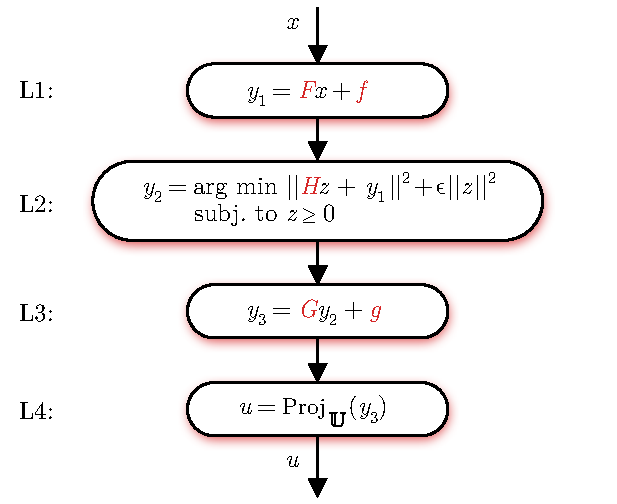
\includegraphics[scale=0.8]{../images/chap4_nn_arch.pdf}  
		\caption{A pQP neural network architecture tailored to MPC. The variables in red are weights to be adjusted during training.}
		\label{fig:nnArchitecture}
	\end{center}
\end{figure}

%Let the chosen number of decision variables in the pQP be $z \in \mathbb{R}^{n_z}$. We choose $L \in \mathbb{R}^{n_z \times n_z}$ to be square, and therefore $F \in \mathbb{R}^{n_z \times n}$, $f \in \mathbb{R}^{n_z}$. Moreover, $G \in \mathbb{R}^{m \times n_z}$ and $g \in \mathbb{R}^{m}$. If $n_z \ge n$, the first layer lifts the input data into a higher dimensional space before it is passed through the optimization layer. A last affine function then projects it onto the control space. These facts will be later employed to analyze the representative power of the network.
Let $\hat\pi : x \mapsto u$ be the pQP NN map defined by the composition of the layers in Figure~\ref{fig:nnArchitecture}, and whose parameters to be trained are $F \in \mathbb{R}^{n_z \times n_x}$, $f \in \mathbb{R}^{n_z}$, $H \in \mathbb{R}^{n_z \times n_z}$, $G \in \mathbb{R}^{n_u \times n_z}$ and $g \in \mathbb{R}^{n_u}$. The final goal is to tune these to fit a dataset of the form 
\begin{equation}
	\{(x(0)_i, u_{0,i}^\star)\}_{i=1}^d
\end{equation}
composed of initial conditions $x(0)$ and the first optimal control action $u_0^\star$ coming from \eqref{eq:linearmpc}. Typically, this is done by defining a suitable loss function and minimizing the mismatch between $\hat\pi(x(0))$ and $u^\star_0$, i.e., the control action produced by the pQP NN and the target optimal value. The parameters are then tuned by means of a gradient-based  backpropagation procedure. 

\begin{remark}
	As shown in \cite[Theorem~1]{amos2017optnet}, OptNet layers are differentiable everywhere, but not in a set of measure zero of parameters, where subgradients exist. Since \eqref{eq:pQP} is a particular instance of the OptNet layer, it inherits its properties. Moreover, we assume the set of feasible control actions $\mathbb{U}$ to be a polyhedron. The projection operator in L4 is therefore a quadratic program with $y_3$ as its only parameter and, thus, also an OptNet layer.
\end{remark}

%This process can be carried out via a stochastic gradient descent algorithm applied to an appropriate loss function. Differentiability of all layers is trivial with the exception of the pQP one \citep{gould2016differentiating,amos2017optnet}. Regarding the latter, note that the objective in \eqref{eq:pQP} can be rewritten as
%\begin{equation}
%	\label{eq:idk}
%	V(z) := z'(\epsilon I + L'L)z + (2L'y_1(x))' \, z + y_1(x)'y_1(x)
%\end{equation}
%whose Lagrangian is simply
%\begin{equation}
%	\mathcal{L}(z,\lambda) = V(z) - \lambda'z
%\end{equation}
%The Karush-Kuhn-Tucker (KKT) conditions for primal and dual feasibility, complementary slackness, and stationarity then read 
%\begin{subequations}
%	\label{eq:kkt}
%	\begin{align}
%		& z^\star \geq 0 \\
%		& \lambda^\star \geq 0 \\
%		& \lambda_i^\star z_i^\star = 0, \ \forall i = 1,\dots,n_z \\
%		& 2(\epsilon I + L'L)z^\star + (2L'y_1(x)) - \lambda^\star = 0
%	\end{align}
%\end{subequations}
%where $\lambda_i$ and $z_i$ denote the components of the Lagrange multipliers and decision variables vectors. The following proposition presents the differentiability properties of the pQP layer, and holds since \eqref{eq:pQP} is a particular instance of the \texttt{OptNet} layer \citep{amos2017optnet} with strictly convex objective function.
%
%\begin{proposition}
%	Let $\theta := (L,y_1)$. The parametric solution $z^\star(\theta)$ of \eqref{eq:pQP} is subdifferentiable everywhere in its domain, i.e., $\partial z^\star(\theta) \neq \{ \, \}$, and $\partial z^\star(\theta)$ has a unique element (the jacobian) everywhere but in a set of measure zero.
%\end{proposition}
%As shown in \cite{amos2017optnet}, the relevant gradients with respect to the parameters to be trained can be obtained from the KKT set of equations \eqref{eq:kkt}. Hence, backward passes are possible and backpropagation can be performed to optimize all of the NN parameters.

\subsection{Properties of the approximator}

%Depending on the number of parameters $n_z$, and thus on the size of the NN, the proposed architecture can not only approximate arbitrarely well, but generate exactly any continuous piecewise affine function. The formal statement is presented next.
The authors of \cite{hempel2013every} showed that any continuous PWA function can be obtained as the solution of a particular parametric linear program (pLP) transformed by a linear map. Even though this view could be adopted herein, we instead prove a different result that is enough in the context of linear eMPC.

\begin{theorem}
	(The proposed NN architecture can learn any linear quadratic MPC controller) Let $\hat{\pi}: \mathcal{X} \rightarrow \mathcal{U}$ be the map defined by the composition of all four layers, i.e., $\hat{\pi}(x) := y_4 \circ y_3 \circ y_2 \circ y_1(x)$. Set $\epsilon = 0$, then $\exists F$, $f$, $L$, $G$ and $g$ with appropriate dimensions such that $\forall x \in \mathcal{X}, \ \hat{\pi}(x) = \pi(x)$.
\end{theorem}

\textit{Proof}: Start by condensing the MPC problem $\mathds{P}1$, i.e., using the equality constraints to eliminate all state decision variables except for the initial state $x(0)$. This leads to the following parametric problem
\begin{subequations}
	\begin{align}
		%\mathds{P}1: \min_{X,U} \quad & q(x_H) + \sum_{k=1}^{H-1} l(x_k,u_k) \\
		\mathds{P}2: \min_{U} \quad & U' \, \Lambda \, U + x(0)' \, \Gamma \, U\\
		\text{s.t.} \quad & \Phi \, U \leq  \Omega \, x(0) + \omega \label{eq:constr}
	\end{align}
\end{subequations}
The step by step procedure can be found in \cite{wright2019efficient}. We have that $\Lambda \succ 0$. Problems $\mathds{P}2$ and $\mathds{P}1$ are then equivalent in the sense that the solution $U^\star$ of $\mathds{P}2$ and $\{X^\star,U^\star\}$ of $\mathds{P}1$ share the same $U^\star$ component. Next, calculate the dual problem of $\mathds{P}2$, which is
\begin{equation}
		\label{eq:dualMPC}
		\mathds{D}2: \min_{\lambda \geq 0} \ \frac{1}{4} \, \big[ \lambda'\Phi \, \Lambda^{-1}\Phi'\lambda + \, (4 x(0)'\Omega' +2 x(0)'\Gamma \Lambda^{-1} \, \Phi' + 4 \omega')\lambda + \, x(0)'\Gamma \Lambda^{-1} \Gamma'x(0) \big]
\end{equation}
It is possible to recover the primal optimal solution $U^\star$ from the dual optimal solution $\lambda^\star$ through the stationarity optimality condition of $\mathds{P}2$
\begin{equation}
	\label{eq:stationarity}
	U^\star = -0.5 \, \Lambda^{-1}\Phi' \lambda^{\star} -0.5 \, \Lambda^{-1} \Gamma'x(0)
\end{equation}

%Next, it would be possible to enforce the first two layers to match the dual problem $\mathds{D}2$, and the third to implement \eqref{eq:stationarity} and recover the primal solution. Nevertheless, this would require the third layer to have a so called skip connection directly from the NN input, i.e., access to $x(0)$. We instead define slightly different linear and pQP layers that not only learn $\mathds{D}2$, but also let $x(0)$ pass through them and arrive at the second linear layer.
The above equation is learned by the second linear layer in Figure~\ref{fig:nnArchitecture}. Nevertheless, from \eqref{eq:stationarity} we see that it requires the value of $x(0)$, which is the NN input. It is shown next that with a pQP layer of appropriate size and parameters, it is possible not only to learn \eqref{eq:dualMPC}, but also let the value of $x(0)$ `pass through' the NN and arrive to the second linear layer as needed to retrieve the primal optimal solution.

Let the auxiliary variable $\tilde{L}$ and function $\tilde{y}_1(x) := \tilde{F}x + \tilde{f}$ be the solution to (compare \eqref{eq:idk} and \eqref{eq:dualMPC})
\begin{subequations}
	\label{eq:Landg1}
	\begin{align}
		\tilde{L}'\tilde{L} + \epsilon I & = 0.25 \, \Phi \Lambda^{-1} \Phi' \\
		2 \tilde{L}'\tilde{y}_1(x) & = \Omega \, x(0) + 0.5 \, \Phi \Lambda^{-1}x(0) + \omega %\\
		%y_1(x)'y_1(x) & = 0.25 \, \overline{r}'\overline{R}^{-1}\overline{r}
	\end{align}
\end{subequations}
which leads to $\epsilon = 0$, $\tilde{L} = 0.5 \, (\Phi \tilde{\Lambda})'$, where $\tilde{\Lambda}$ is the unique square root of $\Lambda^{-1}$, guaranteed to exist as $\Lambda^{-1} \succ 0$. Then, $\tilde{y}_1(x) = (\Phi \tilde{\Lambda})^{-1} (\Omega \, x(0) + 0.5 \, \Phi \Lambda^{-1} x(0) + \omega) \implies \tilde{F} = (\Phi\tilde{\Lambda})^{-1}(\Omega+0.5 \, \Phi \Lambda^{-1}), \; \tilde{f} = (\Phi\tilde{\Lambda})^{-1}\omega$. 

Set the first layer weights to $F = [-I \ I \ \tilde{F}]'$ and $f = [\bm{0} \ \bm{0} \ \tilde{f}]'$ so that $y_1(x) = [-x; \ x; \ \tilde{F}x + \tilde{f}]$. Set the weights of the pQP layer \eqref{eq:pQP} to $\epsilon = 0$ and $L = [I \ \bm{0} \ \bm{0}; \, \bm{0} \ I \ \bm{0}; \, \bm{0} \ \bm{0} \ \tilde{L}]$. If we partition the decision variable as $z = [\tilde{z} \ x^p \ x^n]'$, this results in 
\begin{equation}
	% \small
	\label{eq:pQPtilde}
	\min_{\tilde{z},x^p,x^n \geq 0} \, ||x^p - x(0)||^{2} + ||x^n + x(0)||^{2} + ||\tilde{L}\tilde{z} + \tilde{y}_1(x)||^{2} 
\end{equation}
which is a separable objective in $\tilde{z}$, $\tilde{x}^p$ and $\tilde{x}^n$. Due to the choice of $\tilde{L}$ and $\tilde{y}_1(x)$ in \eqref{eq:Landg1}, the last term of the pQP matches the dual $\mathds{D}2$ with the exception of its constant term -- not relevant for determining the optimal solution. Therefore, we have that $\tilde{z}^\star$ in \eqref{eq:pQPtilde} matches $\lambda^\star$ in $\mathds{D}2$. Regarding $x^{p\star}$, the $n$ optimizer components will satisfy $\forall i = 1,\dots,n$, $x^{p\star}_i = x_i(0)$ if $x_i(0) \geq 0$, else $x^{p\star}_i = 0$. Similarly, $x^{n\star}_i = -x_i(0)$ if $x_i(0) \leq 0$, else $x^{n\star}_i = 0$. Therefore, $x^{p\star} - x^{n\star} = x(0)$, and the output of the pQP layer \eqref{eq:pQPtilde} has the dual optimizer $\lambda^\star$ and the initial condition $x(0)$ encoded in it.

Next set the weights of the second linear layer $y_3$ to $G = [- 0.5 \Lambda^{-1}\Phi' \ -0.5 \Lambda^{-1}\Gamma' \ \ 0.5\Lambda^{-1}\Gamma']$ and $g = \bm{0}$. Therefore, $y_3 = G \, [\tilde{z}^\star \ x^{p \star} \ x^{n\star}]' = G \, [\lambda^\star \ x^{p \star} \ x^{n\star}]' = U^\star$, where equality \eqref{eq:stationarity} was used in the last step. Finally, note that the last layer $y_4 = \text{Proj}_{\mathbb{U}}(y_3)$ will simply evaluate to $y_3$ since $y_3$ is the optimal primal solution $U^\star$, which satisfies the constraints \eqref{eq:constr} and necessarily belongs to $\mathbb{U}$. The theorem then follows from the fact that $x(0)$ in the above calculations can be taken to be any point $x$ in $\mathcal{X}$. $\square$

Exactly matching the original MPC controller would require $L$ to have the same size of $\Phi \tilde{\Lambda}$ and $\epsilon = 0$ as shown. Nevertheless, we are interested precisely in reducing the complexity of the resulting controller through employing less parameters. In this process, choosing a regularizer $\epsilon > 0$ is beneficial since it ensures that the QP is bounded during the training phase for all possible parameters.

Comment: Stability certification

\section{Simulation results}


\subsection{Analysis and controller design}
\label{sec:analysis}
Parallelism is a key concept to increase the efficiency and power levels of electronic converters. Still, this design choice has to be followed by proper current/voltage balancing techniques to ensure that no stage is subjected to a higher electrical stress when compared to the others. 

A schematic representation of a multicell step-down converter is shown in Fig.~\ref{fig:converter}, and its parameters can be found in Table~\ref{tab:param}. The topology features three arms that are connected to a coupled inductor, and an L-C output filter. All self inductances are assumed equal $L_1 = L_2 = L_3 = L_{s}$, and all mutual inductances have value $L_m$. The switches of each arm operate in a complementary fashion at a fixed frequency $f = \,$15 kHz, and with variable but constrained duty cycle $0 \leq d_i \leq 0.9, \, i=1,2,3$. Let the average voltage applied by the arms over one switching period be denoted by $v_i := d_i V_{in}, i=1,2,3$. In order to ease the analysis, we apply the Lunze transform $\Psi$ to all variables, decomposing the phase voltages and currents into differential and common mode components
\begin{equation}
	% \begin{bmatrix}
	%     i_{dm1} \\ i_{dm2} \\ i_{cm}  
	% \end{bmatrix} 
	% := \Gamma 
	% \begin{bmatrix}
	%     i_{1} \\ i_{2} \\ i_{3}
	% \end{bmatrix}
	\begin{bmatrix}i_{dm1} & i_{dm2} & i_{cm}\end{bmatrix}' := \Psi \, \begin{bmatrix}i_{1} & i_{2} & i_{3}\end{bmatrix}' \\
\end{equation}
\begin{equation}
	% \begin{bmatrix}
	%     v_{dm1} \\ v_{dm2} \\ v_{cm}  
	% \end{bmatrix} 
	% := \Gamma 
	% \begin{bmatrix}
	%     v_{1} \\ v_{2} \\ v_{3}
	% \end{bmatrix}
	\begin{bmatrix}v_{dm1} & v_{dm2} & v_{cm}\end{bmatrix}' := \Psi \, \begin{bmatrix}v_{1} & v_{2} & v_{3}\end{bmatrix}' 
\end{equation}
where $\Psi = (1/3) \, [2 \, -1 \, -1; \, -1 \ \, 2 \, -1; \, 1 \ \, 1 \ \, 1]$.

The control input is defined as $u := [v_{dm1} \; v_{dm2} \; v_{cm}]'$ and the continuous-time state vector, by appending the output voltage to the transformed currents $x := [i_{dm1} \; i_{dm2} \; i_{cm} \; v_{out}]'$. By using Kircchoff's circuit laws, a linear model of the form $\dot{x} = A_{ct} x + B_{ct} u$ can be derived with
\begin{equation}
	\small
	A_{ct} = 
	\begin{bmatrix}
		\frac{-R}{L_s - L_m} & 0 & 0 & 0 \\
		0 & \frac{-R}{L_s - L_m} & 0 & 0 \\
		0 & 0 & \frac{-R}{L_s + 2L_m + 3L_f} & \frac{-1}{L_s + 2L_m + 3L_f} \\ 
		0 & 0 & \frac{3}{C_o} & \frac{-1}{R_o C_o}
	\end{bmatrix}
\end{equation}
\begin{equation}
	\small
	B_{ct} = 
	\begin{bmatrix}
		\frac{1}{L_s-L_m} & 0 & 0\\
		0 & \frac{1}{L_s-L_m} & 0 \\
		0 & 0 & \frac{1}{L_s + 2L_m + 3L_f} \\ 
		0 & 0 & 0
	\end{bmatrix}
\end{equation}
Finally, discretization at frequency $f$ is carried out using the zero-order hold method, yielding $x_{k+1} = A x_{k} + B u_{k}$.

The control goal is to regulate the output voltage $v_{out}$ to 300$\,$V while maintaining the phase currents balanced at all times, which translates to driving the differential currents to zero. More specifically we have the following  fixed reference $x_{eq} = [0 \; 0 \; 16 \; 300]'$ with $u_{eq} = B^{\dagger}(I-A)x_{eq}$, where $B^\dagger$ is the pseudo-inverse of $B$. Moreover, the controller approximation procedure must not incur a steady-state error larger than 200$\,$mA for $i_{dm1}$ and $i_{dm2}$, and 5\% for the common mode component $i_{cm}$ and output voltage $v_{out}$. The chosen MPC cost function was
\begin{equation}
	J = \sum_{k=0}^{H-1} (||x_{k}-x_{eq}||_Q^2 + ||u_{k}-u_{eq}||_R^2) \, + \, ||x_{N}-x_{eq}||_P^2
\end{equation}
where $Q = \text{diag}(10, \, 10, \, 0.1, \, 0.1)$, $R = 0.1 \, I$, $P$ is the solution to the associated the discrete-time algebraic Riccati equation, and $H=10$. For all time instants, box state constraints were imposed $\begin{bmatrix}-5 & -5 & -10 & -20\end{bmatrix}' \leq x_{k} \leq \begin{bmatrix}5 & 5 & 30 & 400\end{bmatrix}^{\prime}$ and polyhedron constraints on the controls $H_u \, u_k \leq h_u$ that simply mapped the duty cycle saturation to the Lunze domain. Due to the polytopic input constraints, the system cannot be decomposed into three decoupled parts as the structure of matrices $A_{ct}$ and $B_{ct}$ suggest. Furthermore, the standard terminal set constraint was imposed on $x_H$, defined as the invariant set associated to the unconstrained infinite-time problem formulation.


\begin{figure}[!t]
	\centering
	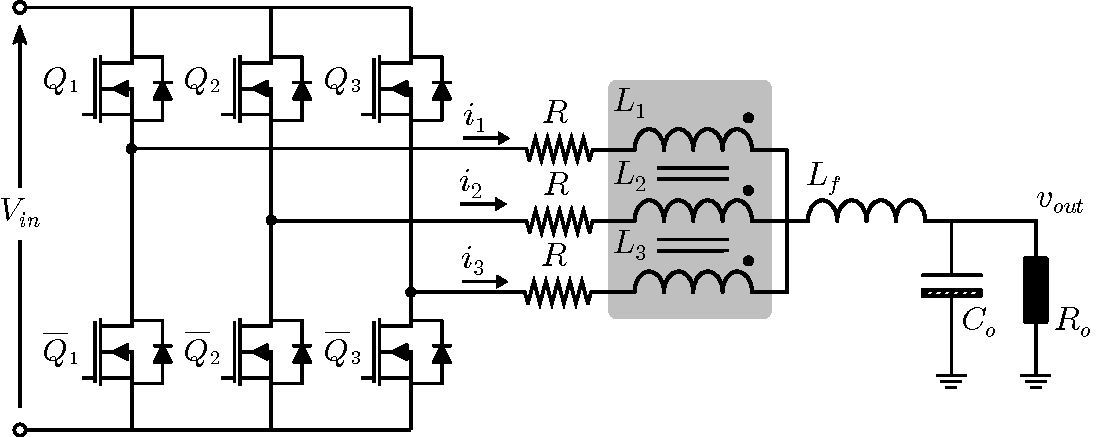
\includegraphics[width=0.7\linewidth]{../images/chap4_simres_multicelldcdc}
	\caption{Photos of the AHU room depicting the air ducts (top), the supply and return water pipes (top and bottom), and the three-way valve servomotor (bottom).}
	\label{fig.asd}
\end{figure}


\begin{table}[b]
	\begin{center}
		\caption{DC-DC converter parameters} \label{tab:param}
		\begin{tabular}{cccccccc}
			\hline 
			$V_{in}$ & $L_{s}$ & $L_{m}$ & $R$ & $L_f$ & $C_o$ & $R_o$ & \\\hline
			350$\,$V & 4$\,$mH & -2$\,$mH & 10$\,$m$\Omega$ & 270$\, \mu$H & 20$\, \mu$F & 6.25$\, \Omega$\\ \hline
		\end{tabular}
	\end{center}
\end{table}


\subsection{Learning the optimal controller}
With the aid of the Multi-Parametric Toolbox (MPT) (\cite{herceg2013multi}), the optimal eMPC solution $\bm{\pi}(x)$ was calculated and consisted of 2'337 critical regions. By counting the number of parameters necessary to describe each halfspace and control gain, the memory requirement of this PWA function was found to be 518$\,$kB. In the previous calculation, a 4 byte representation was considered for both integers and floating point numbers.

Next, 5'000 samples were randomly acquired from the eMPC controller using a uniform distribution. The first and second components of the sampled control moves had considerably smaller amplitudes compared to the third due to the structure of the Lunze transform $\Psi$. The dataset labels $\{\text{u}_i\}_{i=1}^{5000}$ had therefore to be scaled to ensure a similar learning of all control components. Moreover, instead of $\text{Proj}_{\mathbb{U}}(y_3)$, the last NN layer was simplified to $y_4 = \Psi \, \text{sat}(y_3)$ with saturation limits $0$ and $0.9 \, V_{in}$. This clearly guarantees control feasibility without the need of a second quadratic program. NN approximators were trained using \texttt{PyTorch} and the \texttt{OptNet} framework \citep{amos2017optnet}. A mean squared error loss function was minimized by employing the Adam algorithm, mini-batch stochastic gradient descent with batch size $50$, and $150$ epochs. The size $n_z$ of the pQP layer was varied from 1 to 7 and a total of 10 models were trained for each size; the lowest obtained losses are shown in Figure~\ref{fig:lossGraph}. On average, training a model required 42~minutes on a 3.1 GHz Intel Core i7 machine without GPU acceleration, and 23~minutes with a single NVIDIA Tesla T4 graphics card. The learned parameters were then exported to MATLAB in order to calculate the PWA solution of the pQP layer. 


\begin{figure}[h]
	\vspace{35pt}
	\begin{center}
		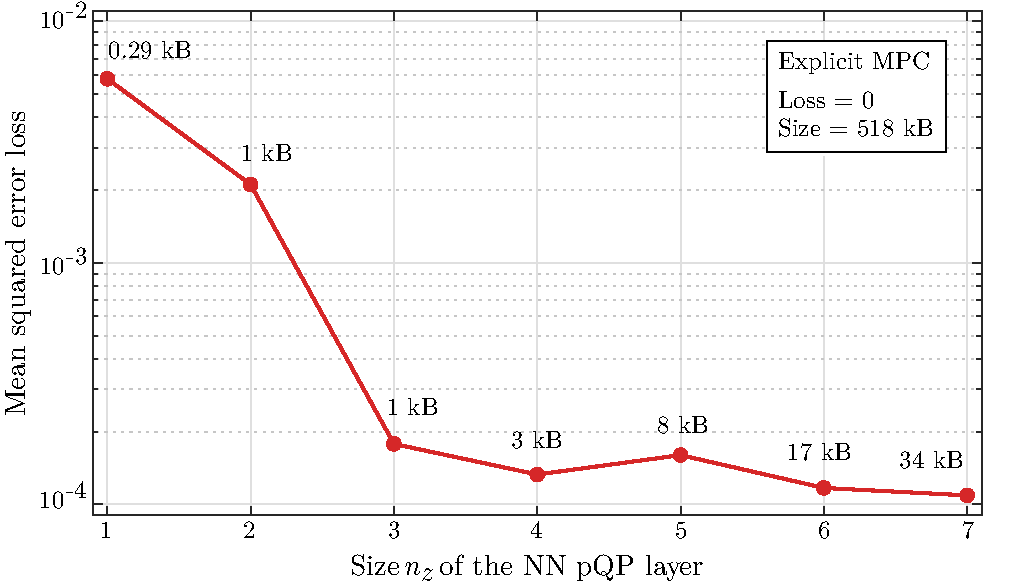
\includegraphics[scale=0.5]{../images/chap4_sim_res_loss_weight.pdf}    % The printed column width is 8.4 cm.
		\caption{Neural network training loss as a function of the	pQP layer size, and storage requirements associated with their PWA representations.} 
		\label{fig:niceSlices}
	\end{center}
\end{figure}

\begin{figure}[h]
	\vspace{35pt}
	\begin{center}
		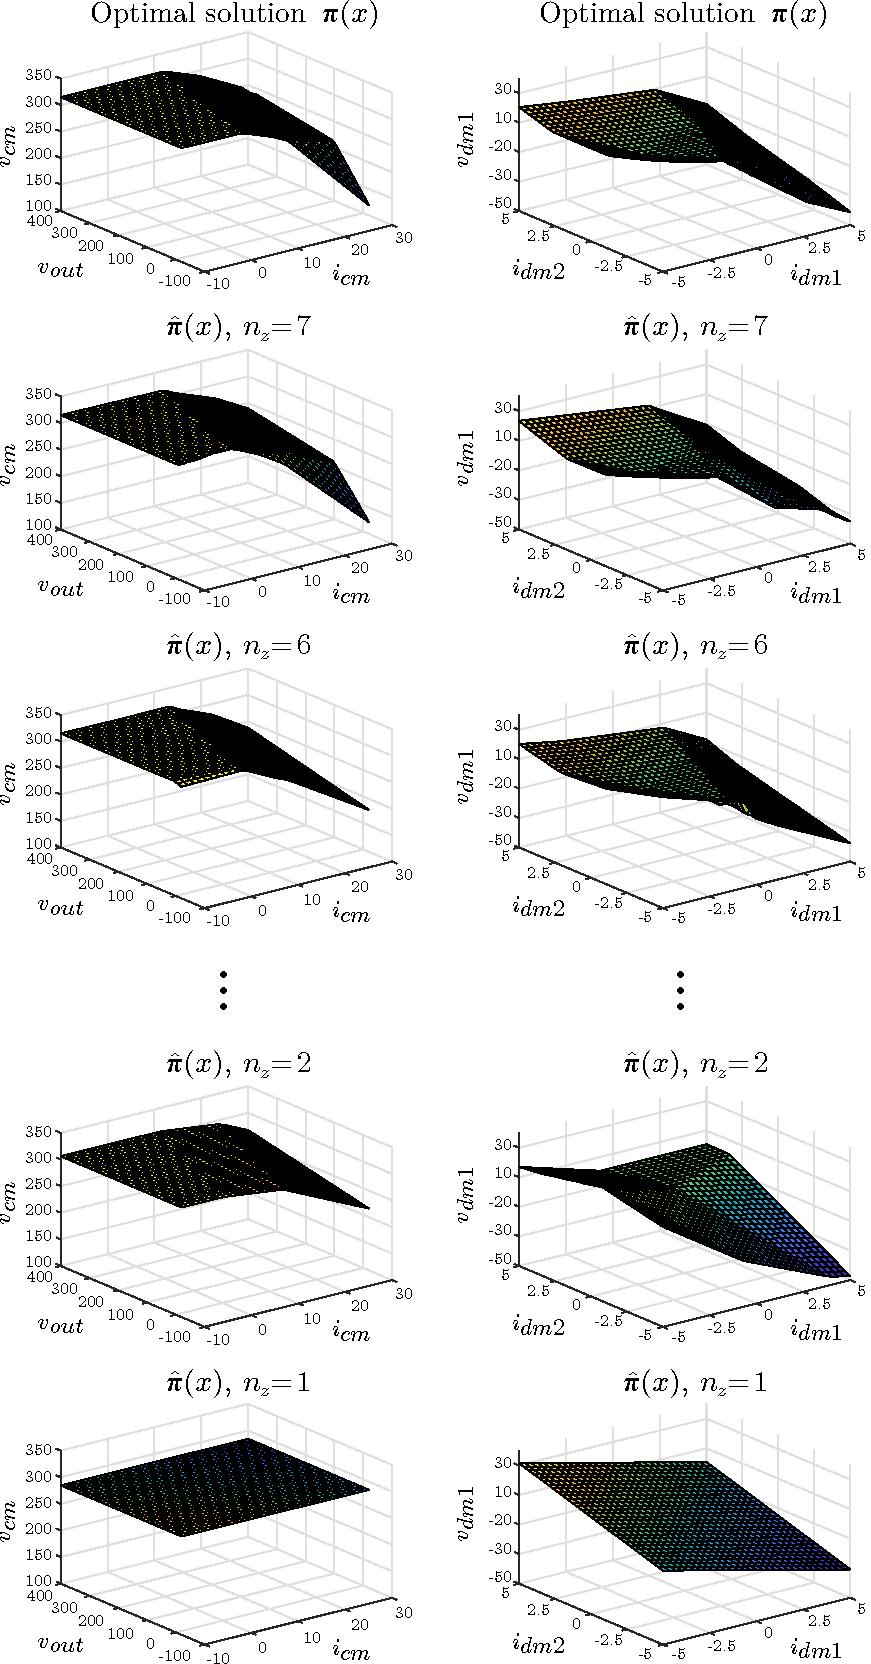
\includegraphics[scale=0.65]{../images/chap4_simres_surfs.pdf}    % The printed column width is 8.4 cm.
		\caption{Slices of the optimal eMPC controller $\bm{\pi}(x)$ and several PWA NN approximations $\hat{\bm{\pi}}(x)$. The left plots are associated to $v_{cm}$ and the right plots, to $v_{dm1}$.} 
		\label{fig:niceSlices}
	\end{center}
\end{figure}

An increase in the $n_z$ size clearly expands the representation capabilities of the neural network. This however does not always translate to a decrease in the final loss since the training process is affected by the weights initialization among other factors. Although not monotonic, we see a decrease of the overall training loss in Figure~\ref{fig:lossGraph} as $n_z$ grows. In order to validate the models, the start-up response of the converter was analyzed under all 7 different approximate controllers, and only the two largest ones ($n_z=$~6 and $n_z=$~7) met the target specifications given in Section~\ref{sec:analysis}. We refer to these two solutions as the \textit{viable learned controllers}. Slices of their control surfaces are shown in Figure~\ref{fig:niceSlices}, and a phase portrait of the closed-loop system evolution over 50 steps starting from four initial conditions is depicted in Figure~\ref{fig:plot1}. A summary of the two viable learned controller features is presented in Table~\ref{tab:sec}, including the number of polytopic regions, the storage requirements, the worst-case computation time\footnote{Before proceeding to implementation, a further speed up would be possible through the methods listed in the Introduction.} and the steady state (SS) error for $i_{cm}$ and $v_{out}$ -- both clearly always equal. Even though four initial states were given, the systems always converged to the same points and, hence, only one SS error is reported. Plus, the storage numbers also take into account all the remaining layers parameters. Analyzing the obtained results we see that the approximations drastically reduced the storage requirements by 93.4\% and 96.7\% and sped up the average evaluation time by 83.7\% and 88.4\%, respectively for the $n_z=$~7 and $n_z=$~6 cases. The closed-loop trajectories with the proposed $\hat{\bm{\pi}}(x)$ remained reasonably close to the scenario with the optimal $\bm{\pi}(x)$, converging to nearby equilibrium points. In practice, steady-state errors could be completely removed by using the tools mentioned in Section~\ref{sec:deployment}.

\section{Experimental results}


A schematic representation of the buck converter considered in this work is shown in Figure~\ref{fig:buck} and its parameters are found in Table~\ref{tab:param}. $V_{IN}$, $V_D$, $L$, and $C$ refer respectively to the input voltage, the diode forward drop, the inductance and the capacitance; whereas $R_{ON}$, $R_L$, $R_C$ and $R_{O}$ refer to the switch on-resistance, the inductor parasitic resistance, the capacitor parasitic resistance, and the output load.

We choose as state variables the inductor current and the output voltage
\begin{equation}
	x = \begin{bmatrix} x_1 \\ x_2 \end{bmatrix}
	= \begin{bmatrix} i_L \\ v_O \end{bmatrix}
\end{equation}


%\begin{table}[b]
%	\begin{center}
%		\caption{Parameters of the DC-DC converter} 
%		\begin{tabular}{ccccc}
%			\specialrule{.15em}{.1em}{.1em} 
%			$V_{IN}$ & $V_{OUT}$ & $V_{D}$ & $L$ & $C$ \\ 
%			\specialrule{.05em}{.1em}{.1em}
%			15$\,$V & 5$\,$V & 0.1$\,$V & 10$\,$mH & 56$\, \mu$F \\ \specialrule{.05em}{.1em}{.1em} \\
%			\specialrule{.15em}{.1em}{.1em}
%			$R_{ON}$ & $R_{L}$ & $R_{C}$ & $R_{O}$ & $f_{\text{sw}}$ \\
%			\specialrule{.05em}{.1em}{.1em}
%			5$\,$m$\Omega$ & 2$\,\Omega$ & 330$\,$m$\Omega$ & 100$\,\Omega$ & 20$\,$kHz \\ 
%			\specialrule{.05em}{.1em}{.1em}
%		\end{tabular}
%	\end{center}
%	\label{tab:param}
%\end{table}

\begin{table}[b]
	\begin{center}
		\caption{Parameters of the DC-DC converter} 
		\begin{tabular}{cccccccccc}
			\specialrule{.15em}{.1em}{.1em} 
			$V_{IN}$ & $V_{OUT}$ & $V_{D}$ & $L$ & $C$ & $R_{ON}$ & $R_{L}$ & $R_{C}$ & $R_{O}$ & $f_{\text{sw}}$ \\
			\specialrule{.05em}{.1em}{.1em}
			15$\,$V & 5$\,$V & 0.1$\,$V & 10$\,$mH & 56$\, \mu$F &
			5$\,$m$\Omega$ & 2$\,\Omega$ & 330$\,$m$\Omega$ & 100$\,\Omega$ & 20$\,$kHz \\ 
			\specialrule{.05em}{.1em}{.1em}
		\end{tabular}
	\end{center}
	\label{tab:param}
\end{table}

\begin{figure}[t]
	\centering
	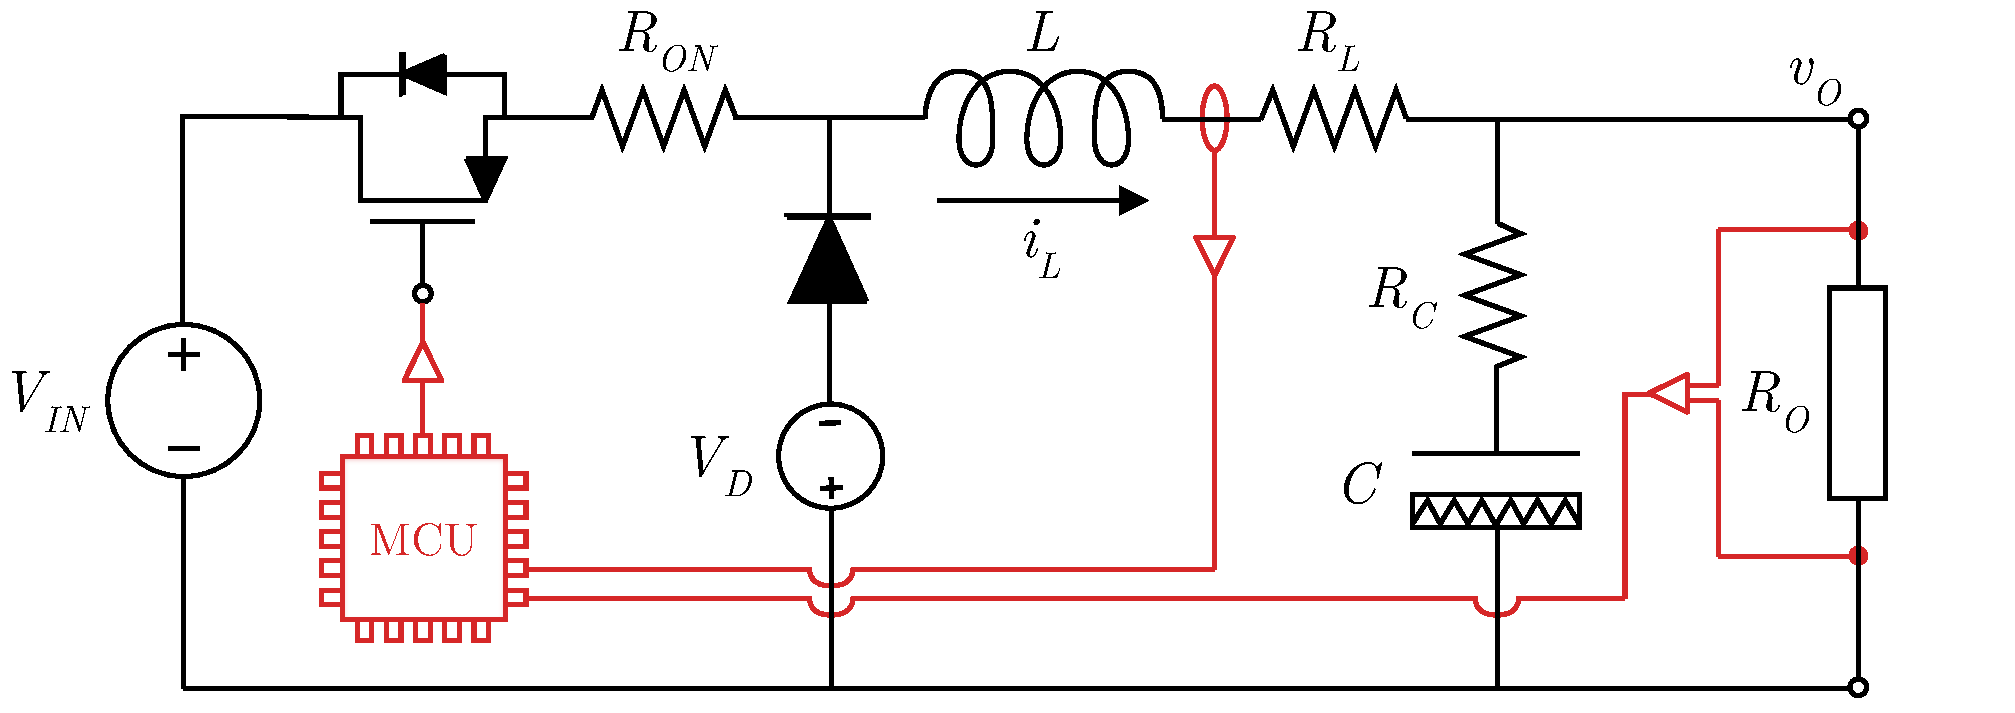
\includegraphics[width=0.8\linewidth]{../images/chap4_buck_schematic.pdf}
	\caption{A circuit diagram of the buck converter including its parasitic resistances and the diode forward voltage drop. The feedback loop is closed by the MCU, which implements our proposed PWA-NN controller.}
	\label{fig:buck}
\end{figure}


The power switch is operated at a constant frequency $f_{\text{sw}}$ and variable duty cycle, which is taken to be the control variable $u = \delta$. Following the classical time-averaging technique, Kircchoff's circuit laws are used to derive differential equations for both when the switch is open, and when it is closed. The expressions can be found in Appendix~\ref{ap.A}. Averaging these equations with $\delta$ as a weight yields

\begin{subequations}
	\begin{flalign}
		\dot{x}_1 = & \small{-\frac{R_L}{L}x_1 - \frac{1}{L}x_2 + \frac{V_{IN}+V_D}{L}u - \frac{R_{ON}}{L} x_1 u - \frac{V_D}{L} \label{eq.x1}} && \\[5pt]
		\dot{x}_2 = & \small{-\frac{R_C R_O R_L C + R_O L}{(R_C + R_O) L C}x_1 -\frac{R_C R_O C + L}{(R_C + R_O)L C}} x_2 + \frac{R_C R_O (V_{IN} + V_D)}{(R_C+R_O)L} u  &&\nonumber \\
		&- \frac{R_C R_O R_{ON}}{(R_C + R_O)L} x_1 u - \frac{R_C R_O V_D}{(R_C + R_O)L} \label{eq.x2} && 
	\end{flalign}
\end{subequations}

The expressions above are not linear since the inductor current and the duty cycle multiply each other. As the goal is to design a linear MPC controller, linearization is needed. We first fix the output voltage to the desired value $x_{2eq}$ and solve for the current and duty cycle steady-state values
%
\begin{align}
	x_{1eq} &= \frac{x_{2eq}}{R_O} \label{eq.x1eq}\\[5pt]
	u_{eq} &= \frac{R_O V_D + (R_L + R_O) x_{2eq}}{R_O(V_{IN}+V_D)-R_{ON} x_{2eq}} \label{eq.ueq}
\end{align}

Finally, \eqref{eq.x1} and \eqref{eq.x2} are expanded around $(x_{1eq},u_{eq})$ and the linear terms are kept, leading to the familiar state-space equations
$\dot{x} = A_{ct} x + B_{ct} u$ where
\begin{align}
	A_{ct} & = \begin{bmatrix} 
		-\frac{R_L+R_{ON} u_{eq}}{L} & -\frac{1}{L} \\[5pt]
		-\frac{R_C R_O (R_L C - R_{ON} C u_{eq}) + R_O L}{(R_C + R_O) L C} & -\frac{R_C R_O C + L}{(R_C+R_O) L C}
	\end{bmatrix} 
	\\[5pt]
	B_{ct} & = \begin{bmatrix} 
		\frac{V_{IN} + V_D - R_{ON} x_{1eq}}{L} \\[5pt]
		\frac{R_C R_O(V_{IN}+V_D-R_{ON}x_{1eq})}{(R_C+R_O)L}
	\end{bmatrix}
\end{align}

As a last step, a discrete-time model $x_{t+1} = A x_{t} + B u_{t}$ is obtained by integrating the continuous-time dynamics using the standard zero-order hold method. The chosen discretization frequency was $f_{\text{samp}} = 10\,$kHz, which is also the predictive controller frequency. 

\begin{figure}[!t]
	\centering
	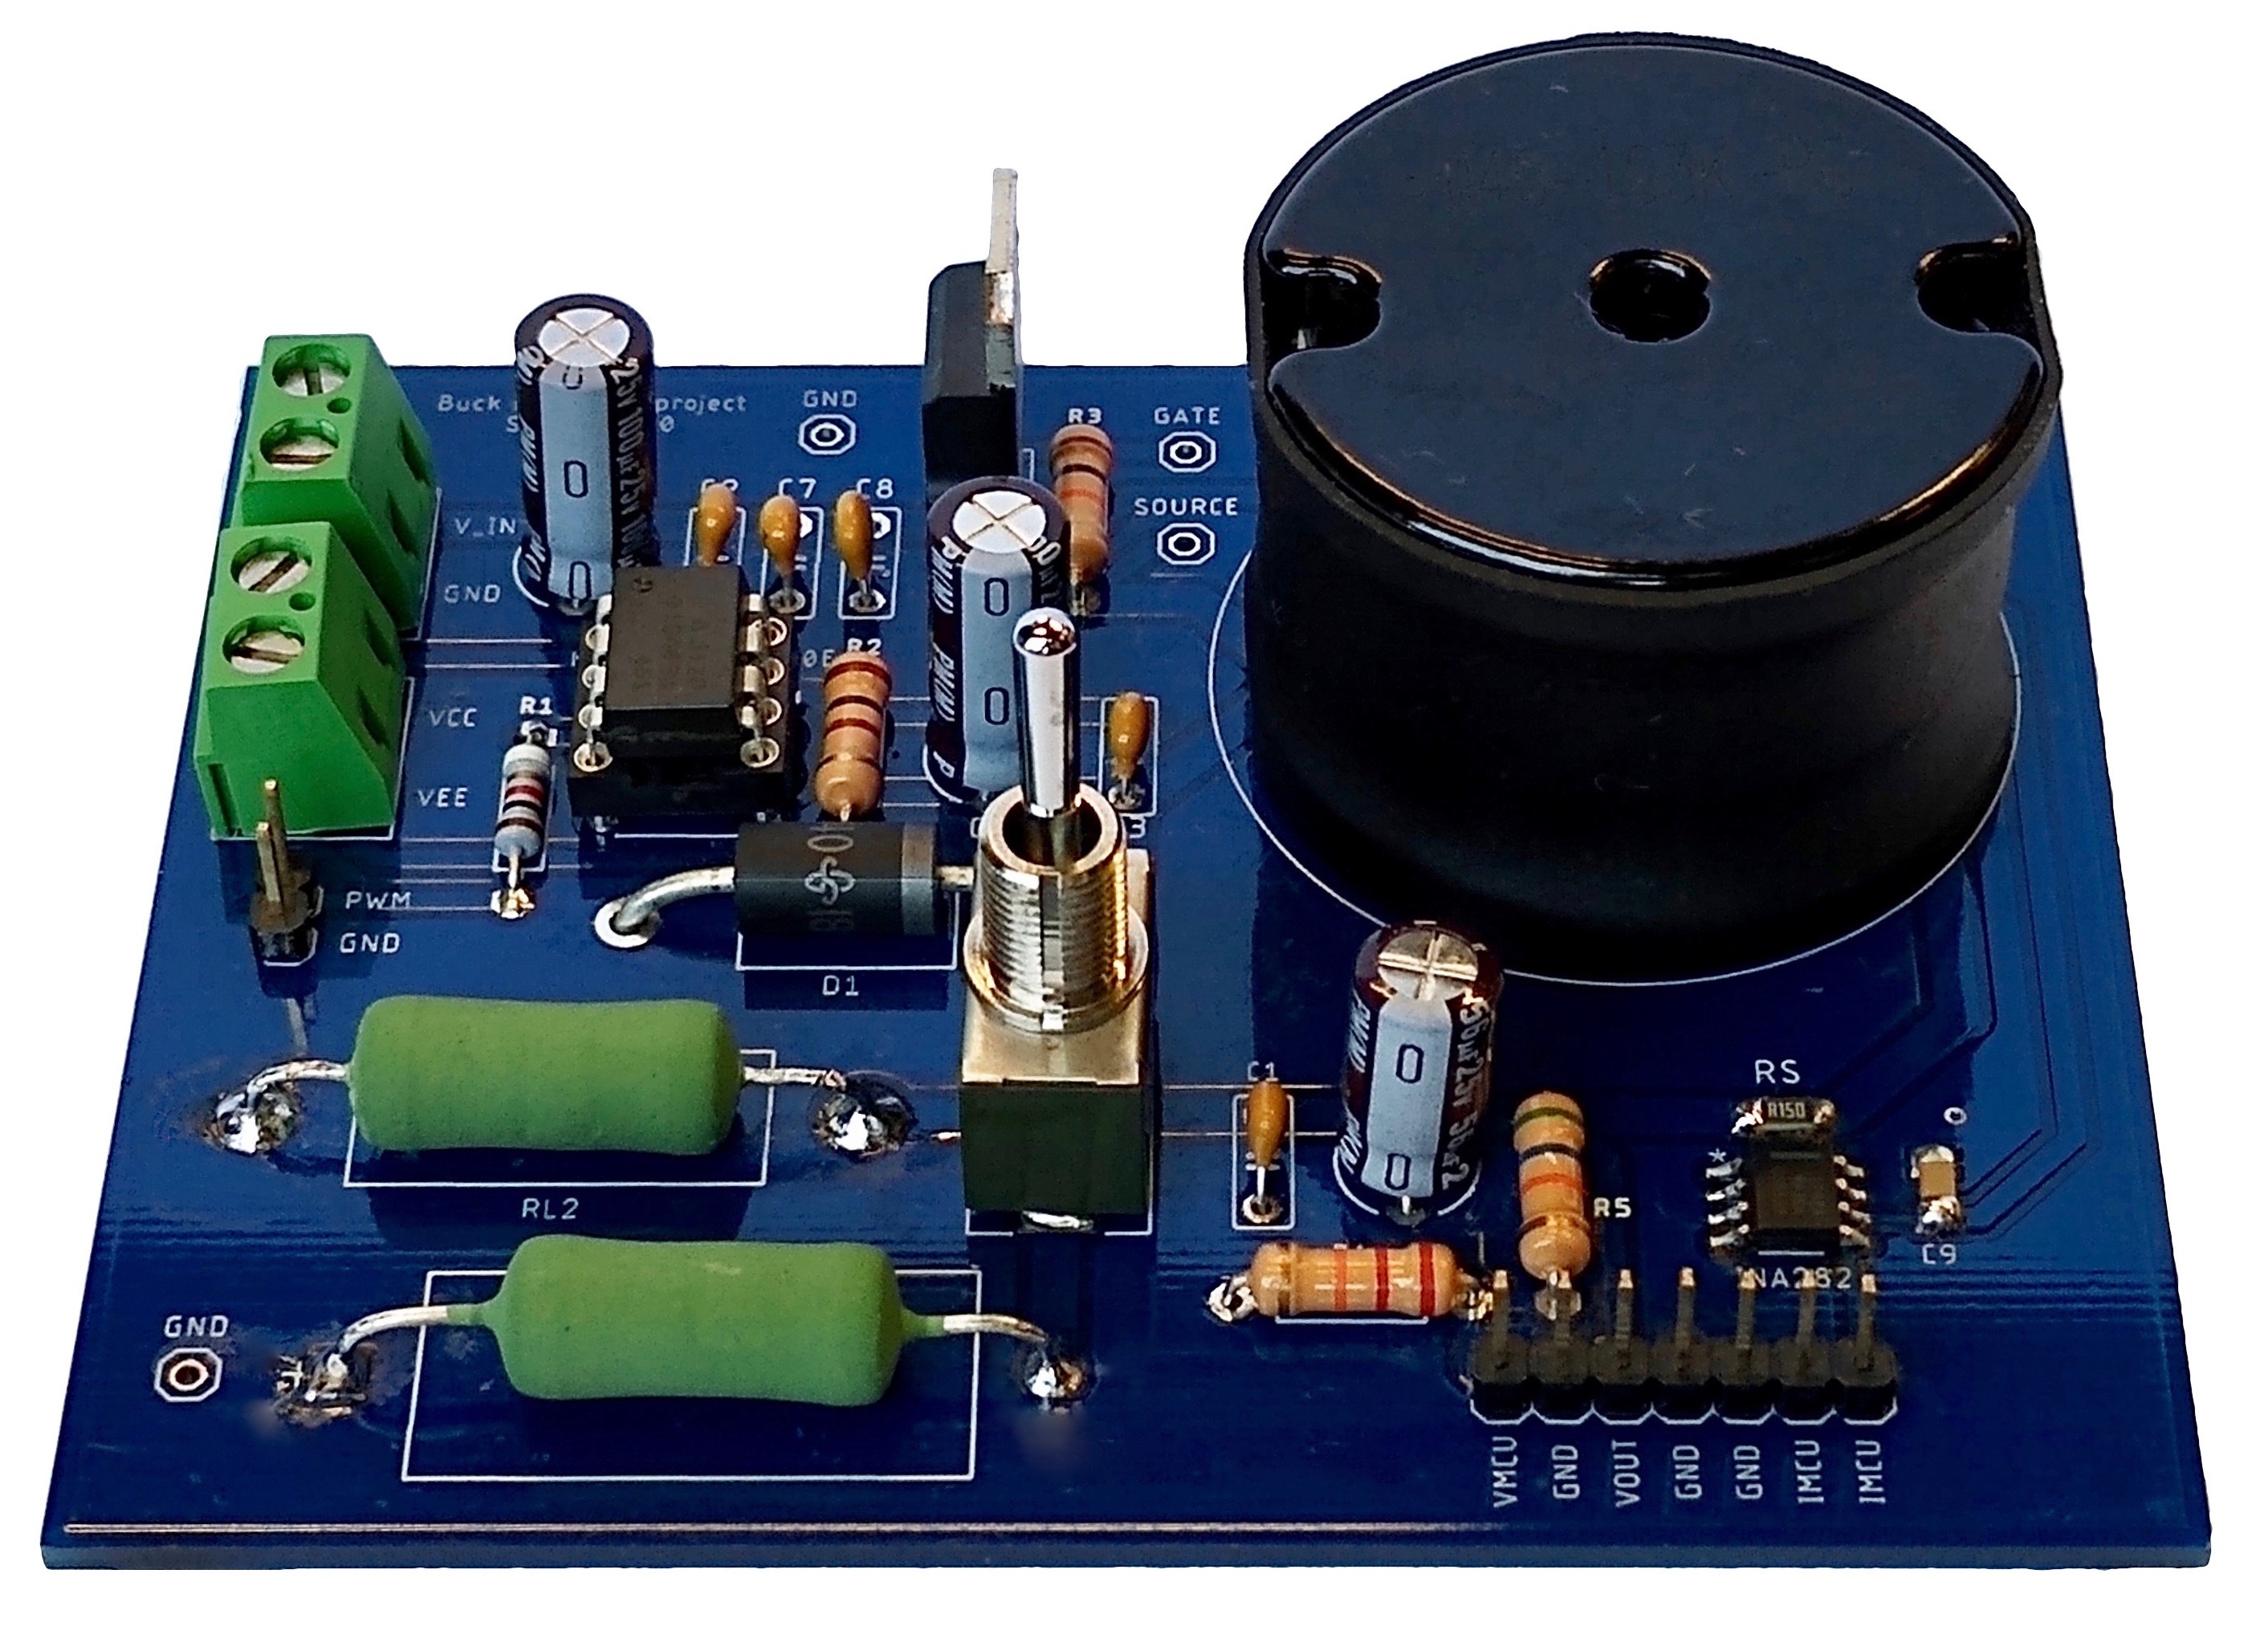
\includegraphics[width=0.7\linewidth]{../images/chap4_buck}
	\caption{Photos of the AHU room depicting the air ducts (top), the supply and return water pipes (top and bottom), and the three-way valve servomotor (bottom).}
	\label{fig.asd}
\end{figure}


The goal is to attain a fast start-up response with as little overshoot as possible and regulate the output voltage $v_O$ to $v_{\text{eq}}=5\,$V. Furthermore, an inductor current constraint of 200$\,$mA and voltage constraint of $7\,$V must be respected at all times. The prediction horizon has to be long enough to yield a large feasible set \cite{rawlings2017model} and we chose $N = 10$ steps. A standard quadratic objective was employed\footnote{In the MPC objective function, the squared weighted norms read as in $\Vert x_t - x_{\text{ref}} \Vert_Q^2 = (x_t - x_{\text{ref}})^\top Q \, (x_t - x_{\text{ref}})$.}, penalizing the deviation of the states and control variable from the reference values $x_{\text{eq}} = \begin{bmatrix} 0.05 & 5 \end{bmatrix}^\top$, $u_{\text{eq}} = 0.3379$. The final optimal-control formulation was
%
\begin{subequations}
	\label{eq:mpcFormulation}
	\begin{align}
		\min_{X,U} \ & \sum_{t=0}^{N-1} \big( \Vert x_t - x_{\text{eq}} \Vert_Q^2 + \Vert u_t - u_{\text{eq}} \Vert_R^2 \big) + \Vert x_N - x_{\text{eq}} \Vert_P^2 \\
		\text{s.t.} \ & \; \forall t = 0,\dots,N-1 \nonumber \\
		& \; x_{t+1} = A x_{t} + B u_{t} \\
		& \begin{bmatrix} i_L^{\text{min}} \\ v_O^{\text{min}}\end{bmatrix}
		\leq x_{t} \leq 
		\begin{bmatrix} i_L^{\text{max}} \\ v_O^{\text{max}}\end{bmatrix} \\
		& \; u^{\text{min}} \leq u_{t} \leq u^{\text{max}} \\
		& \; x_{N} \in \mathcal{X}_N \\
		& \; x_0 = x(0)
	\end{align}
\end{subequations}
with state and control constraints
\begin{align}
	x^{\text{min}} &= 
	\begin{bmatrix} i_L^{\text{min}} \\ v_O^{\text{min}}\end{bmatrix} = 
	\begin{bmatrix} 0 \, \text{mA} \\ 0 \, \text{V}\end{bmatrix} \\[3pt]
	x^{\text{max}} &= 
	\begin{bmatrix} i_L^{\text{max}} \\ v_O^{\text{max}}\end{bmatrix} = 
	\begin{bmatrix} 200 \, \text{mA} \\ 7 \, \text{V}\end{bmatrix} \\[3pt]
	u^{\text{min}} &= 0, \quad u^{\text{max}} = 1 
\end{align}
%
The matrix weights were $Q = \text{diag}(90,1)$, $R = 1$, and $P$ was the solution of the associated discrete-time algebraic Ricatti equation. $\mathcal{X}_N$ was chosen to be the the system's maximal invariant set under the corresponding LQR policy. Both the terminal ingredients ($P$ and $\mathcal{X}_N$) can be easily calculated with the aid of the Multi-Parametric Toolbox (MPT) \cite{mpt} for MATLAB, and are employed to ensure recursive feasibility and closed-loop stability \cite{rawlings2017model}.

As a final step, the MPC controller \eqref{eq:mpcFormulation} was solved off-line using MPT, which yielded a piecewise-affine (PWA) function $\pi(x)$ that maps states directly to optimal control inputs. As well known in the area of explicit model predictive control \cite{alessio2009survey}, this function partitions the space of feasible states $\mathcal{X}$ into regions described by sets of linear inequalities. Then, applying the predictive controller on-line boils down to implementing the look-up table of feedback gains
\begin{align}
	u = \pi(x) = 
	\begin{cases}
		F_1 x + g_1, &\text{if } x \in \text{region } 1 \\
		\quad \; \dots & \qquad \dots \\
		F_M x + g_M, &\text{if } x \in \text{region } M \\
	\end{cases}
	\label{eq.PWA}
\end{align}

As provided by MPT, the computed control policy $\pi(x)$ had $M = 70$ regions, a number too large to be embedded into the target MCU due to the large storage and computational demands (more details are given in Section~\ref{sec.complRed}). These implementation issues motivate the use of our PWA-NN complexity reduction scheme.

\section{Learning a faithful still simpler representation of the controller}
\label{sec.complRed}

Explicit MPC controllers are the exact parametric solution of their optimization counterparts. The geometric landscape depicted by the PWA function $\pi(x)$ is composed of numerous linear pieces patched together. At times, neighboring regions share the same control law and, depending on their arrangement, they could be merged into an equivalent single one. Moreover, the overall surface usually presents two scales of complexity: a general shape and, inspecting it more closely, intricate small details. Based on these observations, it is reasonable to try to reproduce the rough shape of $\pi(x)$ without necessarily replicating its small wiggles.

\subsection{The general architecture}

The architecture of the piecewise-affine neural network used to learn $\pi(x)$ is shown in Figure~\ref{fig:NN}. It has two affine layers (L1 and L3), an optimization problem as the activation layer \cite{amos2017optnet} (L2) and one projection layer (L4) that in this specific case is simply a saturation function. The latter is needed to ensure that the final control values produced by the NN are within the control bounds $0 \leq u \leq 1$. As discussed in \cite{maddalena2019neural}, the motivation behind the structure is that of learning the dual MPC problem: L1 maps the state $x$ to the dual space, where L2 represents the dual optimization problem that is solved, L3 then maps the solution back to the primal space, and finally L4 guarantees it respect the control constraints. 

As opposed to other approaches to learning MPC controllers with NN \cite{zhang2020near,lucia2020deep}, the one explored here can be translated to a \textit{closed-form} piecewise-affine function. More specifically, the parametric quadratic program in layer L2 can be solved off-line after training (e.g. by using MPT), yielding a PWA map of the same form as \eqref{eq.PWA}. The complexity of such function in terms of the number of regions can be adjusted by choosing the size of matrix $H \in \mathbb{R}^{n_z \times n_z}$ inside L2. Fixing $n_z$ also defines the sizes of all remaining trainable parameters highlighted in orange in Figure~\ref{fig:NN}. The result presented next assures the designer that this PWA-NN structure is suitable for any possible predictive controller.


The optimization problem associated with training this NN---in fact, almost any NN architecture---is non-convex. As a consequence, even though there might exist a combination of parameters and weights capable of exactly representing the desired function, reaching them is not an easy task. Since local minima exist, the training process has to be performed multiple times with different initializations. Nevertheless, it is reasonably accepted in the machine learning community that these loss functions possess many high quality local minima, and pursuing a global optimum is irrelevant in this context (see for instance the influential work \cite{choromanska2015loss}).

Theorem~1 establishes that the size of the NN could be chosen to exactly replicate $\pi(x)$, but that would defeat its purpose since the goal is to learn a faithful but \textit{simpler} version of the MPC controller. For this reason, we gradually increased the size $n_z$ during the training process until a desirable approximation quality was attained. From a machine learning perspective, the problem could be interpreted as an approximation one, where the ground-truth is known.


The explicit control law $\pi(x)$ was sampled in order to collect a set of state-control pairs
\begin{equation}
	\{(x_d,u_d) \,|\, d=1,\dots,D\}
\end{equation}
where $x_d$ can be regarded as features and $u_d$ as labels. A total of $D = 5000$ points were gathered randomly using a uniform distribution over the set of feasible states. We highlight that the samples could have been acquired directly from \eqref{eq:mpcFormulation} as well. Next, the data-points were used to train the internal parameters of the layers shown in Figure~\ref{fig:NN}. 

A standard backpropagation approach can be used to iteratively update the NN parameters since, as shown in \cite{amos2017optnet}, optimization layers of this type are differentiable (except on sets of measure zero, where subgradients can be used). The \texttt{PyTorch} and \texttt{OptNet} packages for Python were employed to code the NN and mini-batch stochastic gradient descent was used to train it. The batch size was chosen to be $50$, and the whole dataset was presented to the algorithm a total of $150$ times, i.e., $150$ epochs. In order to achieve a balanced learning throughout the domain, the currents and voltages values that formed the input locations $x_d$ were normalized to a range of $[0,1]$. Furthermore, all trainable weights were initialized randomly. The code was run on a 3.1~GHz Intel Core i7 laptop with 16~GB 2133~MHz of memory. As previously explained, we gradually increased the size $n_z$ of the PWA-NN. Training the network once took approximately $35\,$mins without any GPU acceleration. With $n_z=3$, after only $5$ initializations, the network presented a very low mean squared error training loss: $1.66\times 10^{-7}$. As for the testing phase, we calculated the true outputs $u = \pi(x)$ and the predicted values $\hat{u} = \hat{\pi}(x)$ on a grid of points; the latter were capable of closely reproducing the original controller as shown in the top plots of Figure~\ref{fig:part}.

In order to assess the complexity of the learned controller, its L2 layer was converted into a PWA function using the MPT toolbox. As can be seen from lower plots in Figure~\ref{fig:part}, the number of region was greatly reduced: from 70 in the original partition to 6 in the simplified one, a reduction of 91\%. The total memory required to store the control law parameters was reduced from 9.25~kB to 528~B. The latter quantities were calculated by counting the total number of constants needed to describe all the inequalities that compose the polytopes and the remaining NN layers, and assuming that each of them occupies 1 \textit{word} of space.

\pagebreak

\begin{figure}[p] 
	\vspace*{25pt}
	\centering
	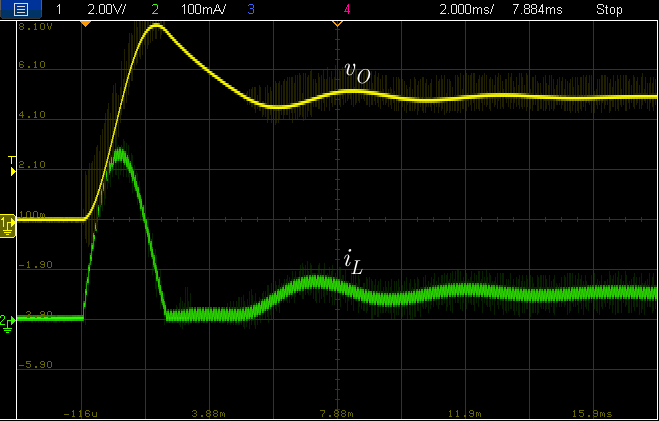
\includegraphics[width=0.65\linewidth]{../images/chap4_scope_ol} \\[10pt]
	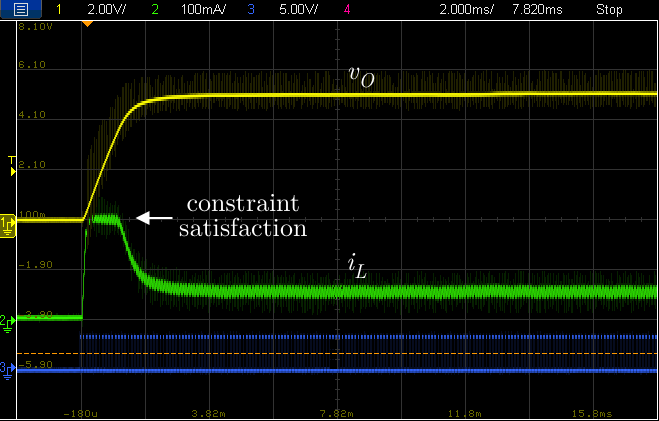
\includegraphics[width=0.65\linewidth]{../images/chap4_scope_cl1} \\[10pt]
	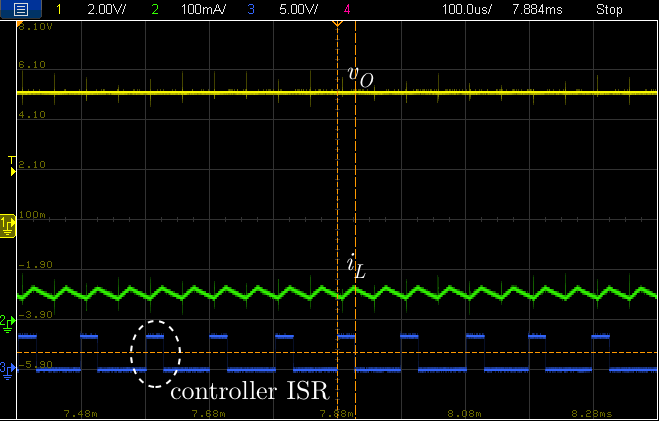
\includegraphics[width=0.65\linewidth]{../images/chap4_scope_cl2}
	\caption{Open-loop start-up response (top), closed-loop start-up response (middle), and a close-up view of the closed-loop start-up response highlighting individual switching cycles and the controller interrupt service routine (ISR) execution time, approximately 27$\;\mu$s.}
	\label{fig.asd}
\end{figure}

\clearpage

\section{Conclusions and outlook}